\chapter{Literature}
\section{Quinachridone (QA)}

\begin{figure}[H]
	\centering
	\begin{subfigure}[b]{0.48\linewidth}
		\centering
		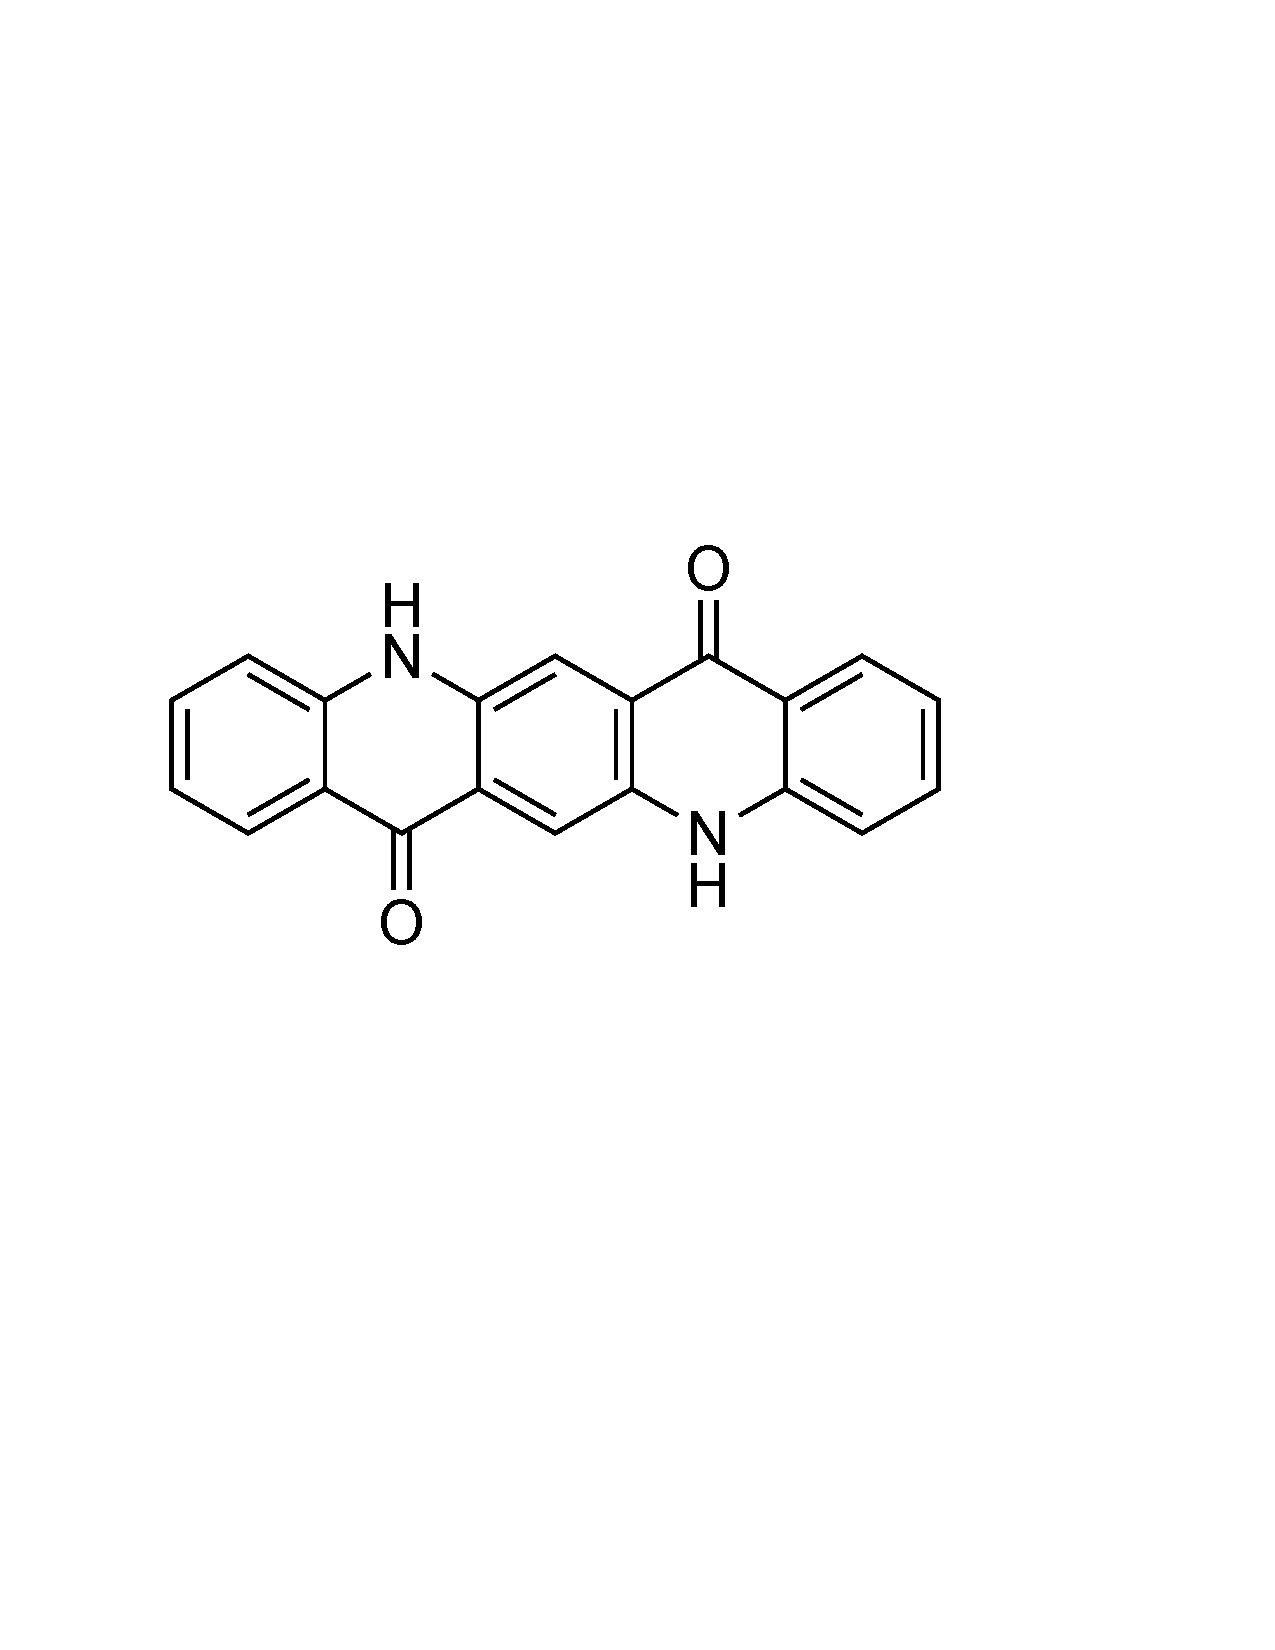
\includegraphics[width=\linewidth]{images/vertiefer/QA.pdf}
		\caption{Skeletal structure}
	\end{subfigure}
	\hfill
	\begin{subfigure}[b]{0.48\linewidth}
		\centering
		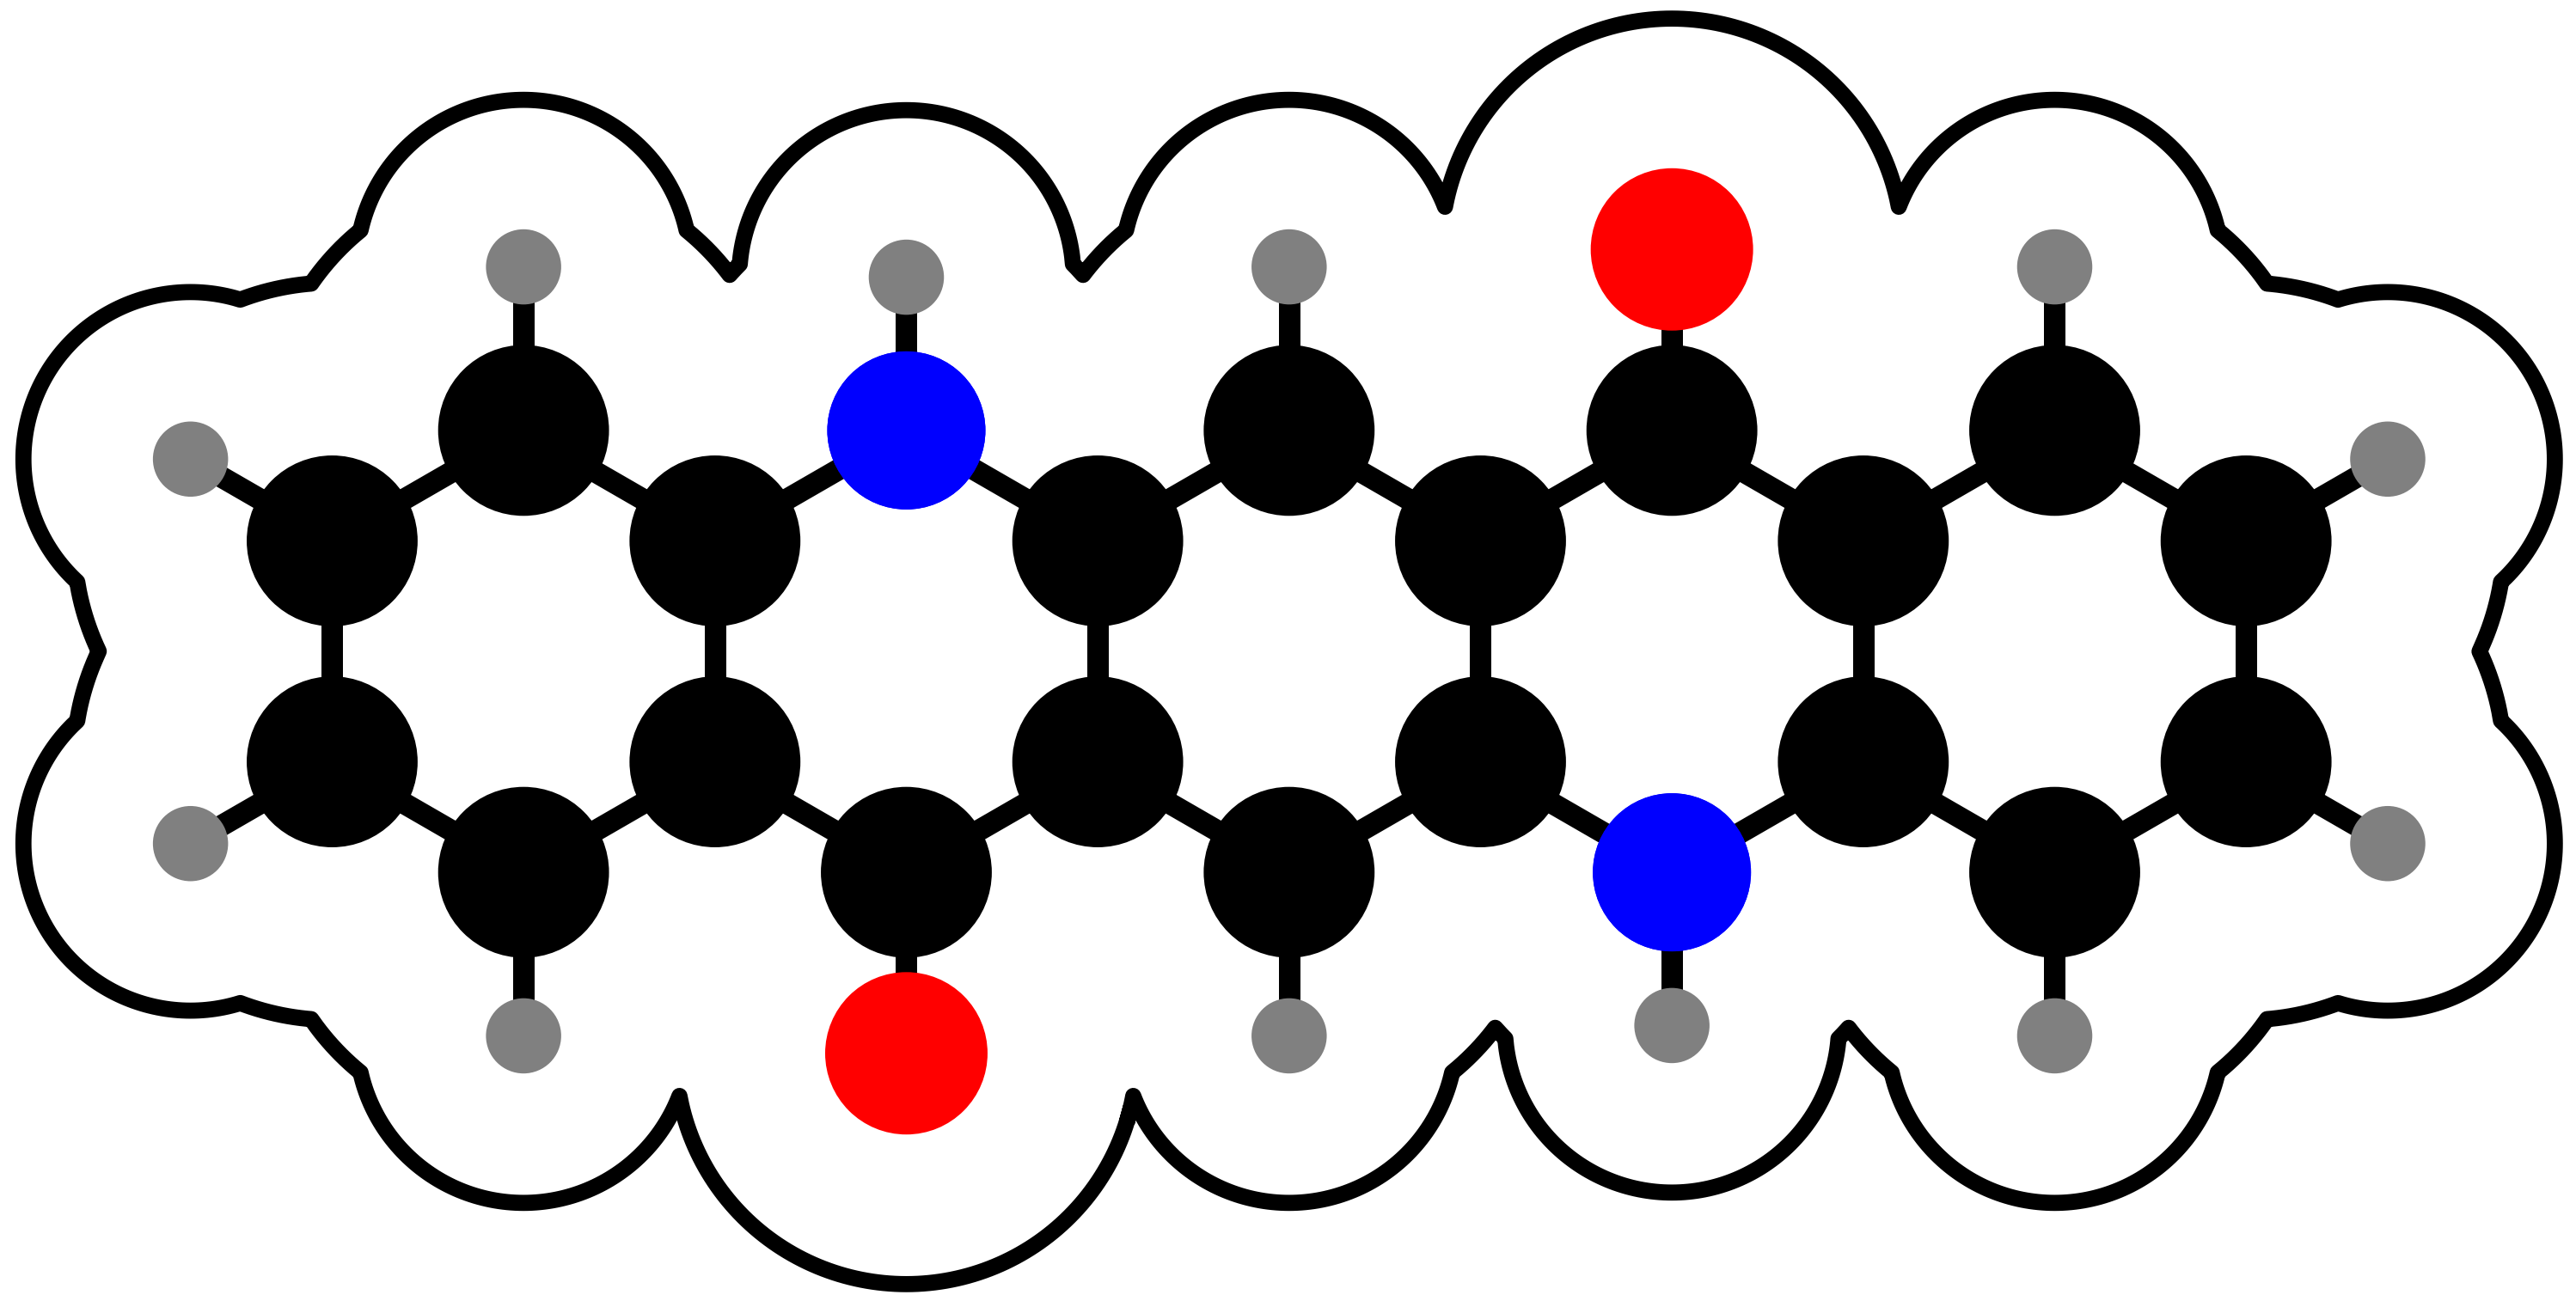
\includegraphics[width=\linewidth]{images/vertiefer/QA_molecule.png}
		\caption{Ball-and-stick model}
	\end{subfigure}
	\caption{Molecular structure of \acf{QA}.}
	\label{fig:QA}
\end{figure}


\section{Structures of Quinachridone (QA) on the Ag(100) surface}

\begin{equation*}
\mathbf{M_\alpha} =\begin{pmatrix}
2 & 1.25 \\
-3 & 4.80 
\end{pmatrix},
\end{equation*}

\begin{figure}[htb]
	\centering
	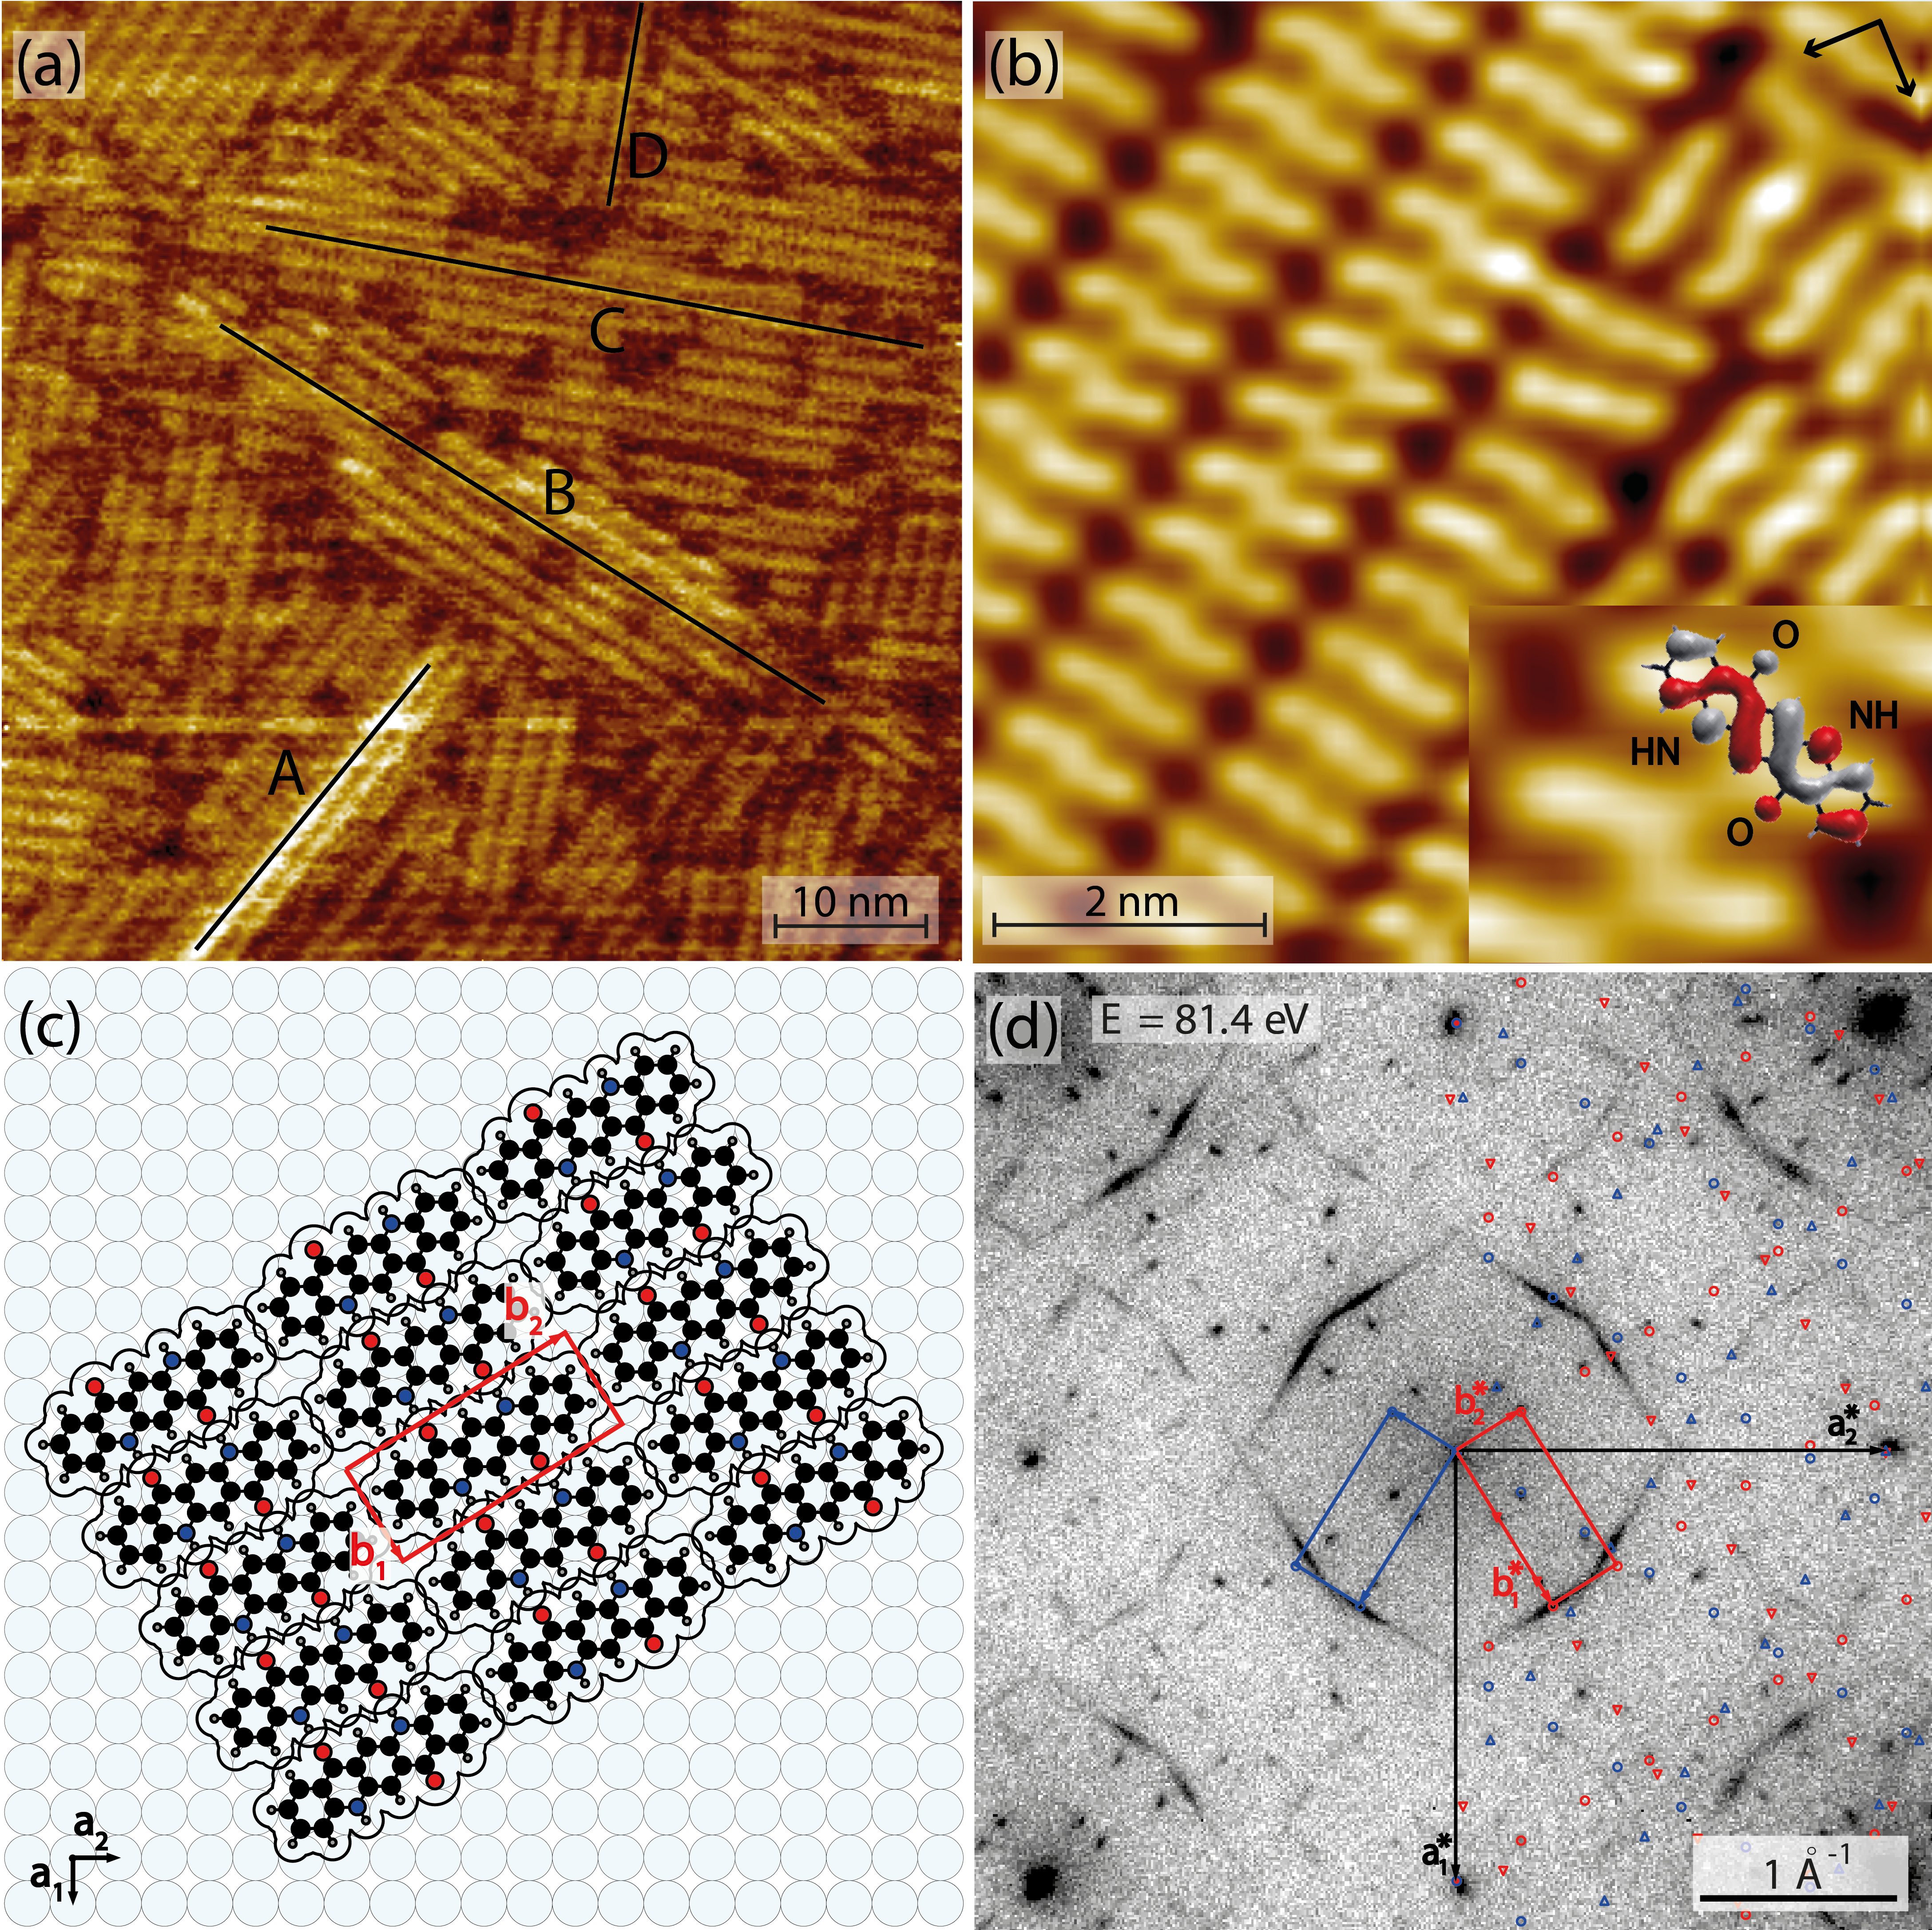
\includegraphics[width=0.8\textwidth]{images/vertiefer/literature_alpha.png}
	\caption{Current structure of complete \ac{ML} of \ac{QA} on Ag(100) in the $\alpha$-phase. The image shows an overview \ac{STM} image (a), a close-up \ac{STM} image of the molecular arrangement (b), the \ac{SPA-LEED} pattern (c) and the structure model (d). The image is taken from reference \cite{Humberg2024}.}
	\label{fig:literature_alpha}
\end{figure}

\begin{equation*}
\mathbf{M_\beta} =\begin{pmatrix}
4 & 3 \\
-5 & 3 
\end{pmatrix},
\end{equation*}

\begin{figure}[htb]
	\centering
	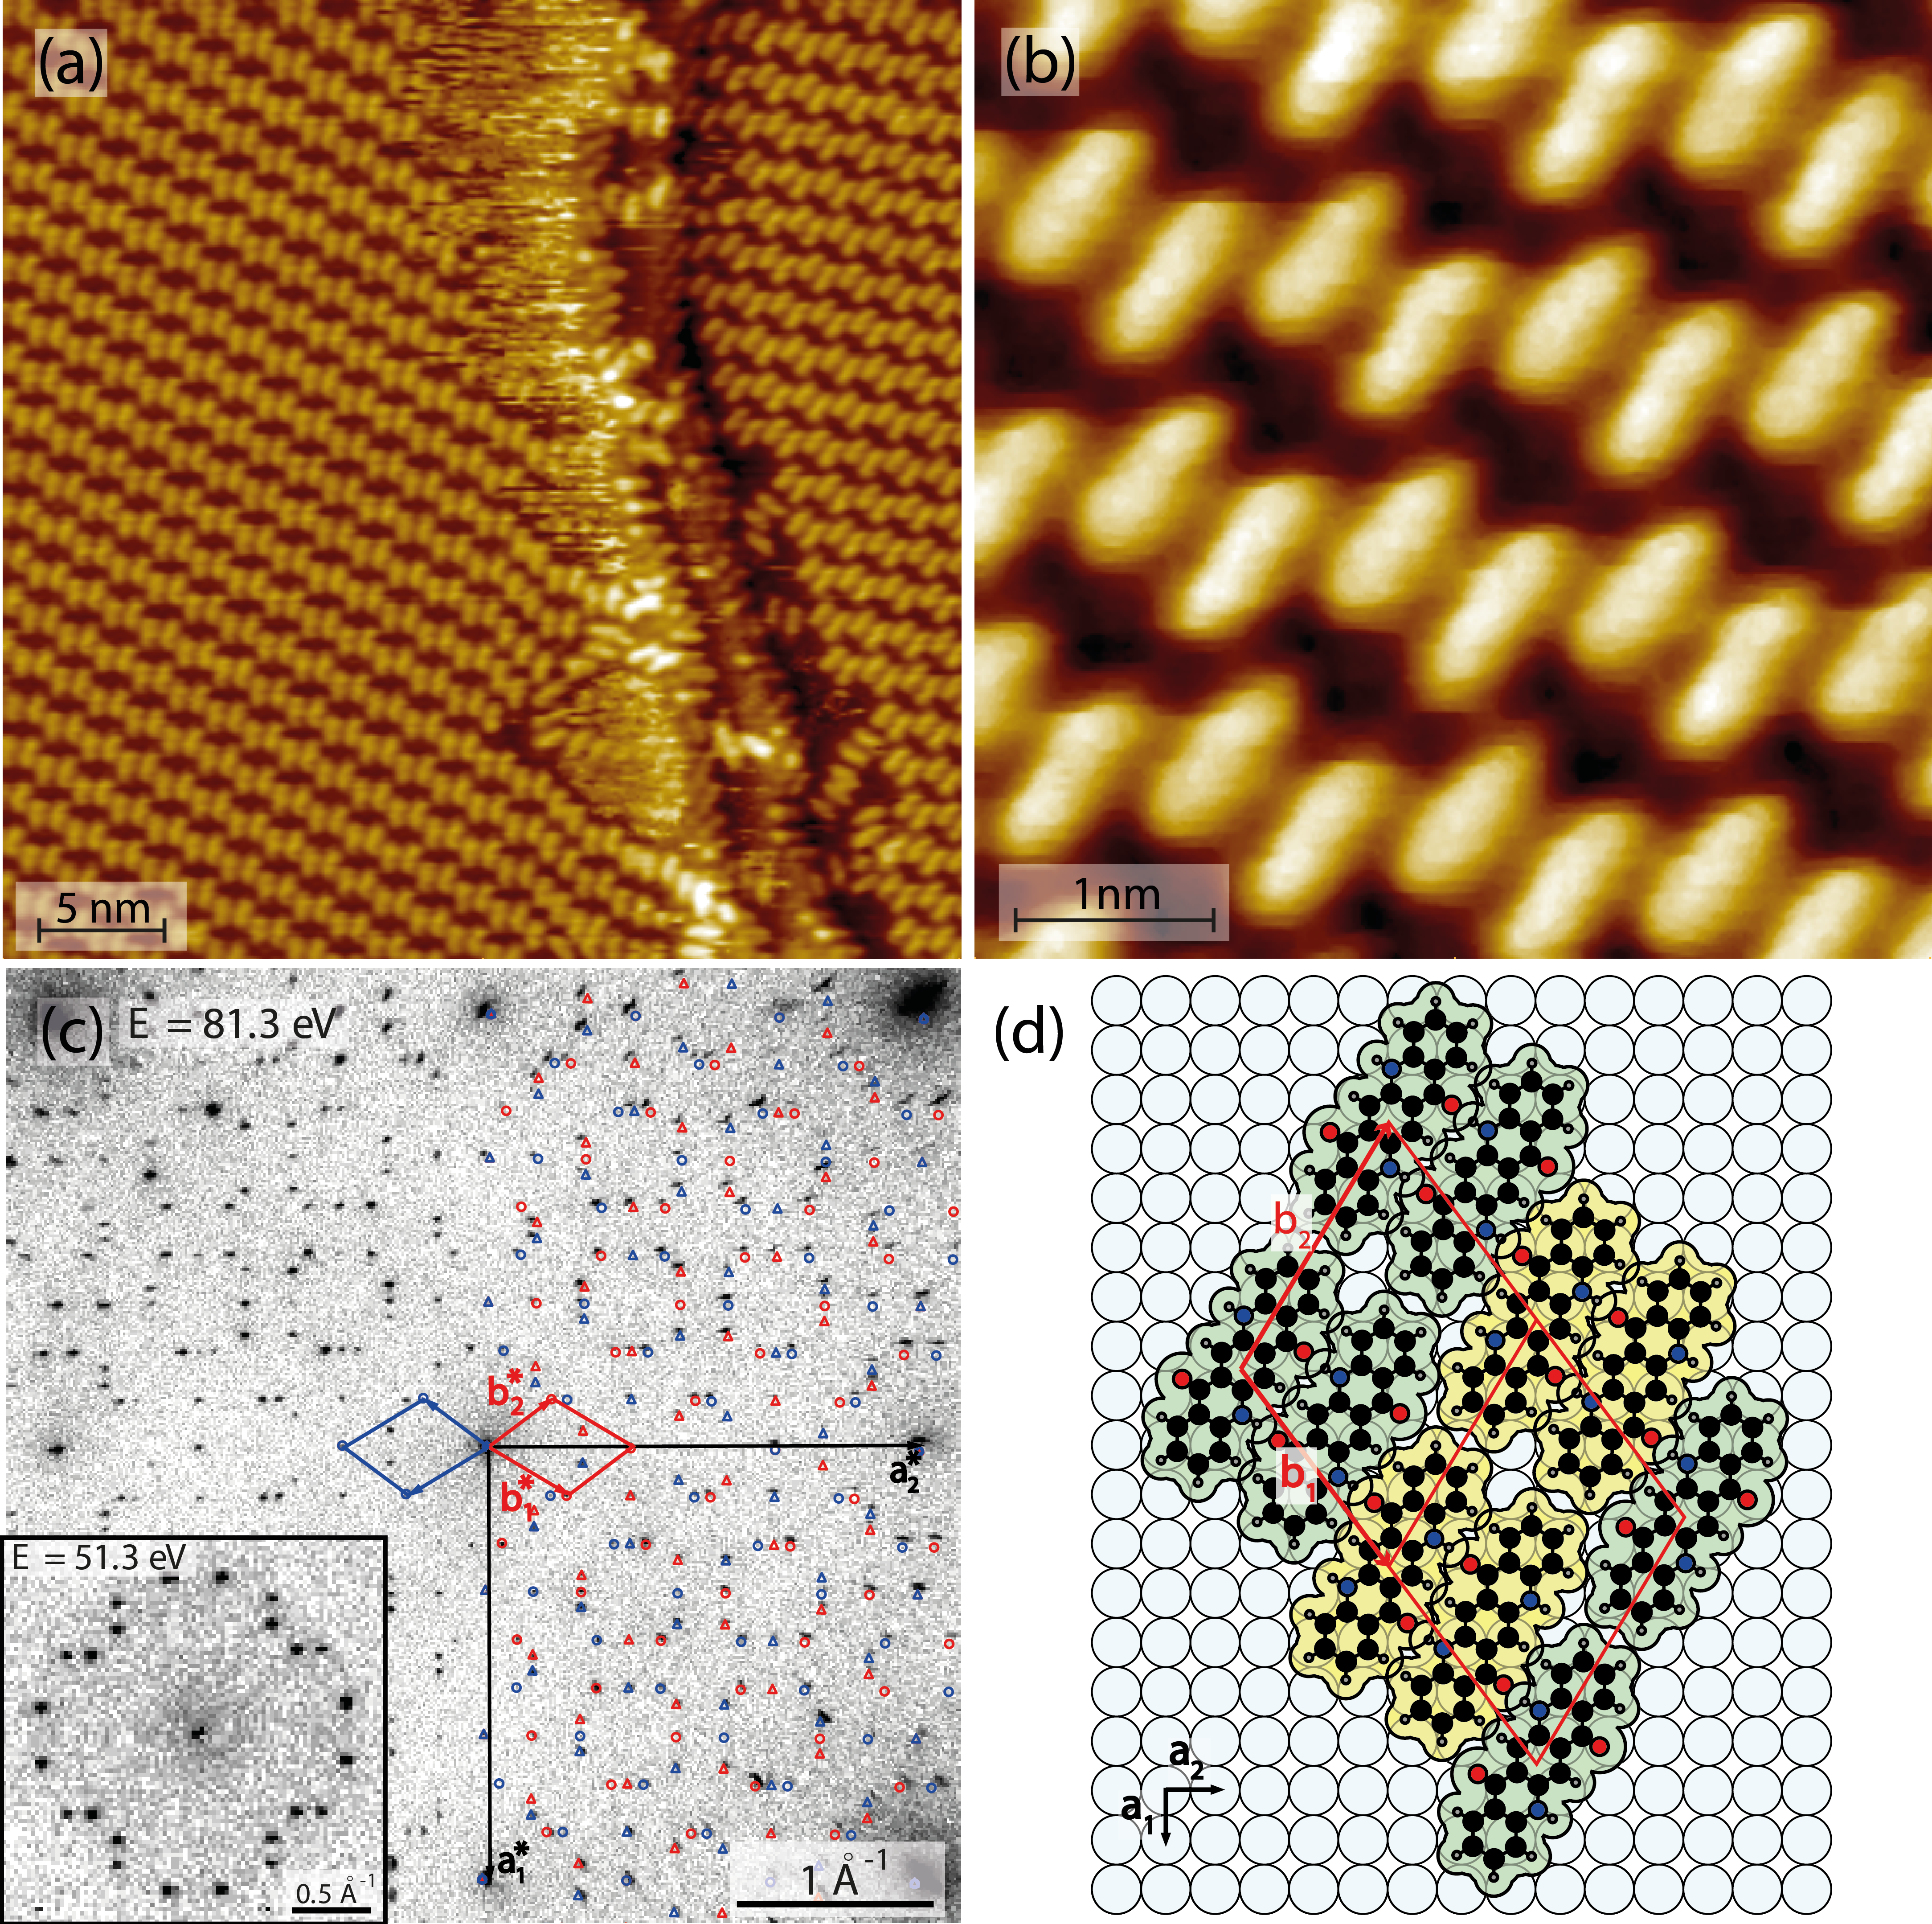
\includegraphics[width=0.8\textwidth]{images/vertiefer/literature_beta.png}
	\caption{Current structure of complete \ac{ML} of \ac{QA} on Ag(100) in the $\beta$-phase. The image shows an overview \ac{STM} image (a), a close-up \ac{STM} image of the molecular arrangement (b), the \ac{SPA-LEED} image (c) and the structure model (d). The image is taken from reference \cite{Humberg2024}.}
	\label{fig:literature_beta}
\end{figure}

\cleardoublepage